%=========================================================
\chapter{Modelo dinámico}	
\label{cap:modDinamico}

	Este capítulo describe en modelo dinámico del sistema. en el se detallan todos los escenarios de ejecución del sistema. La figura~\ref{fig:casosDeUso} muestra el diagrama general del sistema y sus sub sistemas. En este documento solo detallamos los casos de uso del sistema de autenticación.
	
\begin{figure}[htbp]
	\begin{center}
		\fbox{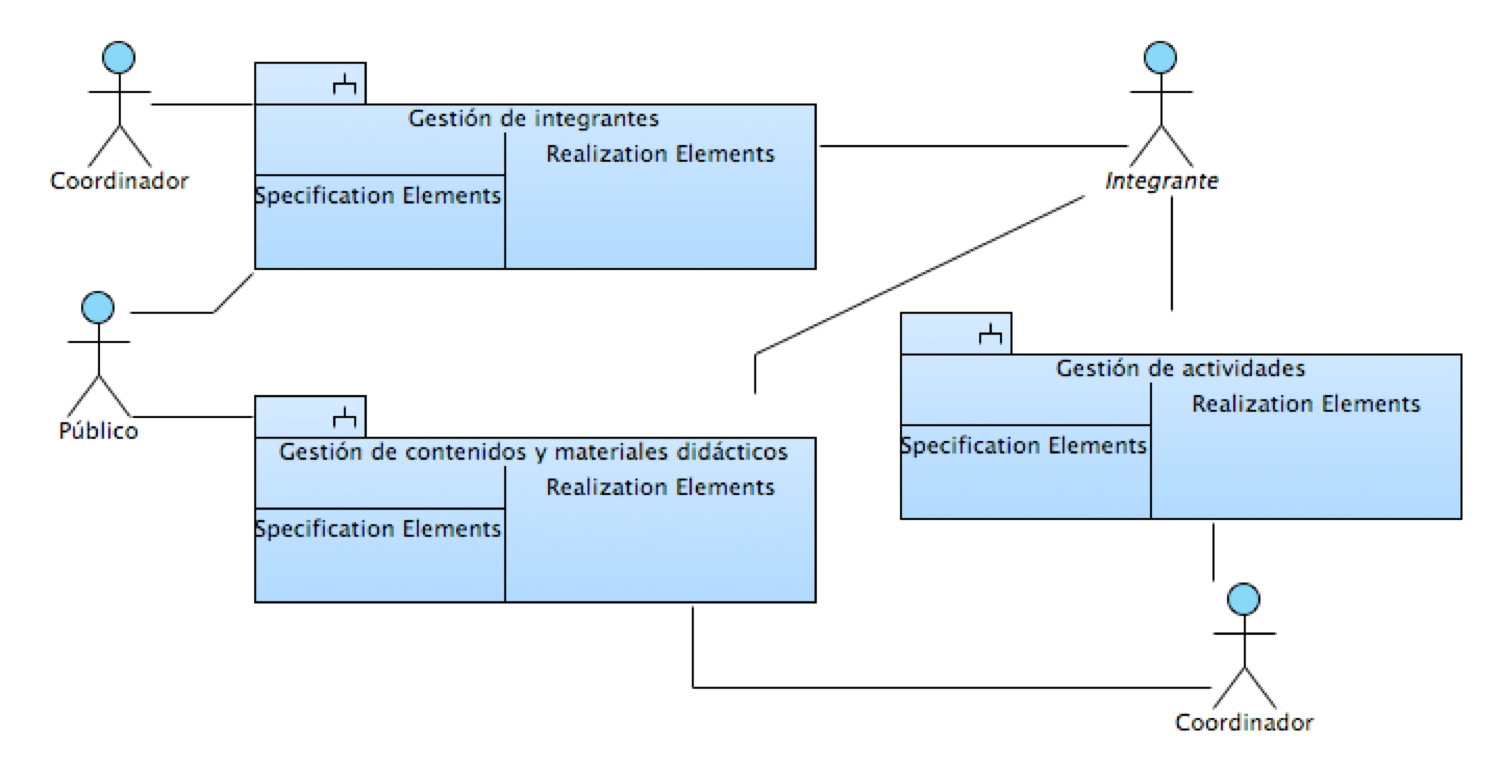
\includegraphics[width=.8\textwidth]{images/casosDeUso}}
		\caption{Diagrama de casos de uso del sistema.}
		\label{fig:casosDeUso}
	\end{center}
\end{figure}

%---------------------------------------------------------
\section{Descripción de actores}

%---------------------------------------------------------
\begin{Usuario}{\hypertarget{tAlumno}{\subsection{Alumno}}}{
		Se refiere a las personas inscritas dentro de algún plan de estudios ofertado en la unidad académica.
	}
	\item[Responsabilidades:] \cdtEmpty
	\begin{itemize}
		\item Mantener actualizados sus datos personales y credenciales de acceso a la aplicación.
		\item Realizar el proceso de autenticación por reconocimiento facial el día de aplicación de los ETS.
		\item Seguir los protocolos de acceso a las instalaciones determinados por la institución y las indicaciones del personal de seguridad.
		\item Asegurarse de usar la aplicación solo en el lugar y momentos adecuados.
	\end{itemize}
	
	\item[Procesos:] \cdtEmpty
	\begin{itemize}
		\item Proceso de autenticación facial: Iniciar sesión en la aplicación, escanear el QR proporcionado y tomar la foto para autenticar su identidad.
		\item Verificación de asistencia: Completar el proceso de autenticación facial para que el sistema registre su asistencia.
		\item Consulta de horarios y ETS: Acceder a la aplicación para revisar detalles sobre horarios de ETS y docentes asignados.
		\item Acceso a resultados y observaciones de acceso: Revisar su historial de accesos, observaciones o restricciones aplicadas en cada caso.
	\end{itemize}
\end{Usuario}

\begin{Usuario}{\hypertarget{tPersonalSeguridad}{\subsection{Personal de seguridad}}}{
		Se refiere a las personas registradas como trabajadores y que permiten o no el acceso a la unidad académica.
	}
	\item[Responsabilidades:] \cdtEmpty
	\begin{itemize}
		\item Supervisar los accesos a las instalaciones en días de ETS, permitiendo solo el ingreso de estudiantes registrados a un ETS.
		\item Consultar los registros de acceso en tiempo real y verificar que los estudiantes cumplan con los horarios permitidos.
		\item Verificar las credenciales físicas y digitales de cada estudiante en caso de ser necesario.
		\item Tomar nota de cualquier incidente o anomalía durante los accesos y registrar observaciones cuando sea necesario.
	\end{itemize}
	
	\item[Procesos:] \cdtEmpty
	\begin{itemize}
		\item Control de acceso: Verificar la autenticación de los estudiantes antes de permitir el ingreso a las instalaciones, revisando que coincidan con los registros del sistema.
		\item Consulta de horarios de ETS y listas de estudiantes autorizados: Revisar los horarios de aplicación y comparar los estudiantes presentes con las listas de acceso.
		\item Gestión de incidentes: Registrar cualquier observación relevante en el sistema si un estudiante no logra autenticar su identidad correctamente o si surgen problemas en la entrada.
		\item Reporte de acceso: Al final de cada jornada de ETS, verificar los registros de acceso y reportar cualquier irregularidad o comentario relevante a la administración del sistema.
	\end{itemize}
\end{Usuario}

\begin{Usuario}{\hypertarget{tDocenteAplicador}{\subsection{Docente aplicador}}}{
		Se refiere a las personas registradas como trabajadores que dan clases a los alumnos y supervisan los ETS asignados.
	}
	\item[Responsabilidades:] \cdtEmpty
	\begin{itemize}
		\item Generar y mostrar el código QR a los estudiantes antes de cada ETS para habilitar la autenticación facial.
		\item Supervisar el proceso de verificación de identidad de los estudiantes y confirmar que todos los presentes hayan completado la autenticación.
		\item Revisar y gestionar las listas de alumnos que presentarán el ETS.
		\item Reportar cualquier irregularidad observada durante el proceso de autenticación o el examen.
	\end{itemize}
	
	\item[Procesos:] \cdtEmpty
	\begin{itemize}
		\item Generación de QR de autenticación: Iniciar la sesión en la aplicación y generar el QR para cada sesión de ETS.
		\item Supervisión de autenticación: Verificar en la aplicación que todos los estudiantes hayan completado el proceso de autenticación mediante el QR y reconocimiento facial.
		\item Consulta de ETS asignados y horarios: Revisar el sistema para conocer los horarios y detalles de los ETS a aplicar.
		\item Registro de asistencia final: Confirmar que todos los estudiantes autenticados están presentes y registrar su asistencia oficialmente.
	\end{itemize}
\end{Usuario}



A continuación se detallan los casos de uso.

%---------------------------------------------------------
% CASOS DE USO

% \IUref{IUAdmPS}{Administrar Planta de Selección}
% \IUref{IUModPS}{Modificar Planta de Selección}
% \IUref{IUEliPS}{Eliminar Planta de Selección}

% 


% Copie este bloque por cada caso de uso:
%-------------------------------------- COMIENZA descripción del caso de uso.

%\begin{UseCase}[archivo de imágen]{UCX}{Nombre del Caso de uso}{
%--------------------------------------
	\begin{UseCase}{CU1}{Iniciar Sesión}{
		Este caso de usos permite al usuario iniciar sesión en el sistema para poder visualizar los Exámenes a Título de Suficiencia (ETS).
	}
		\UCitem{Actor}{\hyperlink{Alumno}{Alumno, Personal de seguridad, Docente}}
		\UCitem{Propósito}{Permitir al usuario ingresar al sistema.}
		\UCitem{Entradas}{Número de boleta (en caso de ser alumno), RFC (en caso de ser del Personal de seguridad o Docente) y Contraseña.}
		\UCitem{Origen}{Teclado}
		\UCitem{Salidas}{-}
		\UCitem{Destino}{Pantalla principal del sistema}
		\UCitem{Precondiciones}{El usuario deberá estar registrado en el sistema SAES.}
		\UCitem{Postcondiciones}{El usuario podrá acceder a la funcionalidad del sistema.}
		\UCitem{Errores}{Es posible que al intentar iniciar sesión se presenten los siguientes inconvenientes: 
			\begin{itemize}
				\item El usuario ingresa sus credenciales incorrecta. 
				\item El usuario no llena todos lo campos obligatorios. 
			\end{itemize}
		}
		\UCitem{Tipo}{Caso de uso primario}
		\UCitem{Observaciones}{}
	\end{UseCase}
%--------------------------------------
	\begin{UCtrayectoria}
		\UCpaso[\UCactor] Introduce su Número de Boleta en caso de ser alumno o su RFC en caso de ser Docente o Personal de seguridad y Contraseña en el sistema vía la  \IUref{IU1}{Pantalla de Inicio de sesión}\label{CU01Login}.
		\UCpaso[\UCactor] Confirma la operación presionando el botón \IUbutton{Iniciar Sesión}.
		\UCpaso Verifica que los datos ingresados coincidan con algún registro guardado dentro del sistema SAES con base en la regla \BRref{BR129}{Determinar.} \Trayref{A} \Trayref{B}.
		\UCpaso Despliega la \IUref{IU02}{Pantalla principal} con la lista de opciones disponible que tiene cada usuario.
	\end{UCtrayectoria}

%--------------------------------------		
		\begin{UCtrayectoriaA}{A}{El Estudiante intenta iniciar sesión , pero el Número de boleta o RFC o contraseña no coincide con algún registro dentro de la base de datos}
			\UCpaso Muestra el Mensaje {\bf MSG1-}``El usuario [{\em Número de Boleta o RFC}] no coincide con ninguna cuenta. Verifique la información e intente de nuevo''.
			\UCpaso[\UCactor] Oprime el botón \IUbutton{Aceptar}.
			\UCpaso[] Termina el caso de uso.
		\end{UCtrayectoriaA}
		

%--------------------------------------
% Puntos de extensión
\subsection{Puntos de extensión}
\UCExtenssionPoint{
	% Cuando:
	Desea conocer las materias cursadas.
}{
	% Durante la región:
	Del paso 4 al paso 9.
}{
	% Casos de uso a los que extiende:
	\hyperlink{CU3.4}{CU3.4 Consultar historial académico}.
}
		
		
		
%-------------------------------------- TERMINA descripción del caso de uso.



